% !TEX encoding = UTF-8
% !TEX TS-program = pdflatex
% !TEX root = ../tesi.tex

%**************************************************************
\chapter{Verifica e validazione}
\label{cap:verifica-validazione}
%**************************************************************

\intro{In questo capitolo viene descritto come sono state affrontate le attività di verifica e validazione del prodotto.}\\

%**************************************************************
\section{Considerazioni}
\label{sec:considerazioni}

Nel piano di lavoro, redatto dal tutor aziendale e approvato dal tutor interno, veniva menzionato lo sviluppo del test automatici come un obiettivo opzionale, preferendo ad essi nuove feature. Per questo, in accordo con il mio tutor aziendale, mi sono dedicato maggiormente all’implementazione e documentazione di esse. Ho comunque avuto modo di effettuare dei test manuali sull’applicativo, verificando il suo corretto funzionamento. I test automatici, che per mancanza di tempo non sono stati sviluppati, verranno implementati successivamente dall’azienda, per provare l’effettiva qualità del software prodotto.

\section{Analisi statica}

Per effettuare l’analisi statica del codice, non sono stati utilizzati particolati strumenti, perché è stato ritenuto che l’IDE PyCharm fornisse aiuti più che sufficienti. PyCharm possiede suggerimenti riguardanti eventuali errori nel codice e miglioramenti per ottimizzare la scrittura del codice.
In particolare, PyCharm segnala, più comunemente:
\begin{itemize}
	\item incoerenza tra tipi di dati coinvolti in un’istruzione se utilizzati i type hint;
	\item codice non raggiungibile dal flusso di controllo;
	\item codice duplicato;
	\item librerie utilizzate ma non dichiarate nei requisiti del progetto;
	\item variabili dichiarate ma non utilizzate;
	\item possibile staticità dei metodi;
	\item metodi dichiarati ma non implementati;
	\item controllo delle librerie importate ma non utilizzate.
\end{itemize}
\noindent
Inoltre, per concludere, PyCharm offre due funzionalità fondamentali, una è la formattazione automatica del codice (ricordando che in python codice mal formattato non viene eseguito) e l’altra è l’importazione e organizzazione di classi, moduli e librerie, sempre automatica.

\section{Analisi dinamica}

Per quanto concerne l’analisi dinamica, ho potuto verificare il codice utilizzando due strumenti fondamentali quali il debugger integrato di PyCharm e la libreria Python logger. I test sono stati tutti effettuati manualmente, a questo fine sono state create tre macchine virtuali connesse nella stessa rete. La prima centralizza i servizi utilizzati, quali redis e rabbitmq, ed il componente denominato master. Le altre due macchine, invece, effettuavano lo scraping utilizzando il componente denominato worker collegandosi ai servizi offerti dalla prima macchina. \newline{}
Al termine di una run di test viene effettuato un lavoro di analisi dei log. Utilizzando una libreria python da me sviluppata, si può ottenere una visualizzazione grafica delle informazioni ritenute interessanti dall'analista, facilitandone il lavoro. Un esempio concreto è l'analisi dell'utilizzo di memoria da parte del modulo durante le varie iterazioni, una rappresentazione grafica può risultare più facilmente intepretabile.

\begin{figure}[!h] 
    \centering 
    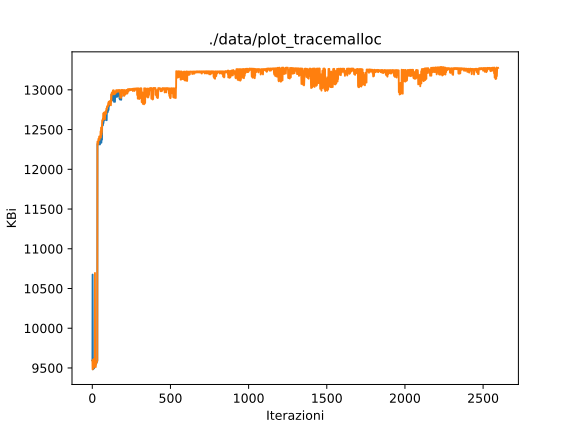
\includegraphics[width=1\columnwidth]{chapter5-verify/tracemalloc.png} 
    \caption{Visualizzazione utilizzo memoria}
    \label{fig:visualizzazione-utilizzo-memoria} 
\end{figure}




